\documentclass[mathserif,hyperref={urlcolor=cyan,colorlinks=true}]{beamer}
\usepackage[utf8]{inputenc}

\usetheme{Warsaw}
%\usetheme{Ilmenau}
%\usetheme{Berlin}

%\usecolortheme{orchid}
%\usecolortheme{rose}
%\usecolortheme{whale}

\usepackage{lmodern}
\usepackage[T1]{fontenc}
\usepackage{textcomp}
\usepackage{multicol}

\usepackage{minted}
\usemintedstyle{monokai}

%\newminted{perl}{fontsize=\fontsize{9}{9}}
\newminted{bash}{fontsize=\fontsize{9}{9}}
\newminted{c}{fontsize=\fontsize{9}{9}}
\definecolor{bgc}{HTML}{272822}

\beamertemplatenavigationsymbolsempty
\setbeamertemplate{footline}{}

\title{XS Accessors\\Under The Hood}
\author{Sergey Aleynikov}
%\institute{Crazy Panda}
\date[August 2016]{YAPC Europe 2016}

\begin{document}{

\begin{frame}
\titlepage
\end{frame}

{
\newminted{perl}{fontsize=\fontsize{9}{9}}
\color{white}
\setbeamercolor{background canvas}{bg=bgc}
%\setbeamertemplate{frametitle}[default][colsep=-4bp,rounded=false,shadow=false]

\begin{frame}[fragile]
\begin{perlcode}
sub make_accessor {
    my ($class, $field) = @_;
 
    *{$class."::".$field} = sub {
        my $self = shift;

        if (scalar @_) {
            return $self->{$field} = $_[0];
        } else {
            return $self->{$field};
        }
    };
}
\end{perlcode}
\pause
basic: Rounded run time per iteration: 3.1598e-07 $\sim$ 3200000/sec
%\pause
hash: Rounded run time per iteration: 2.4837e-08 $\sim$ 40000000/sec
\end{frame}

\begin{frame}[fragile]
\begin{perlcode}
sub make_accessor {
    my ($class, $field) = @_;

    *{$class."::".$field} = sub {
        @_ > 1 ? ($_[0]->{$field} = $_[1]) : $_[0]->{$field}
    };
}
\end{perlcode}
\pause
basic: Rounded run time per iteration: 3.1598e-07 $\sim$ 3200000/sec
better: Rounded run time per iteration: 2.6846e-07 $\sim$ 3700000/sec
\end{frame}

\begin{frame}[fragile]
\begin{perlcode}
sub make_accessor {
    my ($class, $field) = @_;

    *{$class."::".$field} = sub {
        @_ > 1 ? ($_[0]->{$field} = $_[1]) : shift->{$field}
    };
}
\end{perlcode}
\pause
better: Rounded run time per iteration: 2.6846e-07 $\sim$ 3700000/sec
shift: Rounded run time per iteration: 2.4664e-07 $\sim$ 4000000/sec
eval: Rounded run time per iteration: 2.2583e-07 $\sim$ 4400000/sec
\end{frame}

\begin{frame}[fragile]
\begin{multicols}{2}
\begin{bashcode}
perl -MO=Concise,-exec,foo \
 -e 'sub foo{ shift->{foo} }'

1  <;> nextstate(main 1 -e:1) v
2  <0> shift s*



3  <1> rv2hv sKR/1
4  <$> const(PV "foo") s/BARE
5  <2> helem sK/2
6  <1> leavesub[1 ref] K/REFC,1
\end{bashcode}
\columnbreak
%\pause
\begin{bashcode}
perl -MO=Concise,-exec,foo \
 -e 'sub foo{ $_[0]->{foo} }'

1  <;> nextstate(main 1 -e:1) v
2  <$> gv(*_) s
3  <1> rv2av sKR/1
4  <$> const(IV 0) s
5  <2> aelem sKM/DREFHV,2
6  <1> rv2hv sKR/1
7  <$> const(PV "foo") s/BARE
8  <2> helem sK/2
9  <1> leavesub[1 ref] K/REFC,1
\end{bashcode}
\end{multicols}
\end{frame}

\begin{frame}[fragile]
\begin{ccode}
SV* name_sv = ST(0);
SV* key_sv = ST(1);

char* name = SvPV_nolen(name_sv);
CV* cv = newXS_flags(name, accessor, __FILE__, NULL, 0);
\end{ccode}
\pause
\begin{ccode}
#define _XPVCV_COMMON
    union {
    OP *    xcv_start;
    ANY xcv_xsubany;
    }       xcv_start_u;

SvREFCNT_inc_simple_void_NN(key_sv);
CvXSUBANY(cv).any_ptr = key_sv;
\end{ccode}
\end{frame}

\begin{frame}[fragile]
\begin{ccode}
static MGVTBL sv_payload_marker;

char* name = SvPV_nolen(name_sv);
CV* cv = newXS_flags(name, accessor, __FILE__, NULL, 0);

sv_magicext(cv, key_sv,
    PERL_MAGIC_ext, &sv_payload_marker, NULL, 0);
SvRMAGICAL_off(cv);

CvXSUBANY(cv).any_ptr = key_sv;
\end{ccode}
\end{frame}

\begin{frame}[fragile]
\begin{ccode}
char* name = SvPV_nolen(name_sv);
CV* cv = newXS_flags(name, accessor, __FILE__, NULL, 0);

STRLEN len;
char* key_buf = SvPV(key_sv, len);
SV* s_key_sv = newSVpvn_share(key_buf, len, 0);

sv_magicext(cv, s_key_sv,
    PERL_MAGIC_ext, &sv_payload_marker, NULL, 0);
SvREFCNT_dec_NN(s_key_sv);
SvRMAGICAL_off(cv);

CvXSUBANY(cv).any_ptr = s_key_sv;
\end{ccode}
\end{frame}

\begin{frame}[fragile]
\begin{ccode}
XSPROTO(getter) {
    dXSARGS;
    SP -= items;

    SV* self;
    if (items != 1 || !SvROK(self = *++SP)) croak("Oops");

    SV* obj = SvRV(self);
    if (SvTYPE(obj) != SVt_PVHV) croak("Oops");

    SV* key_sv = CvXSUBANY(cv).any_ptr;
    HE* hent = hv_fetch_ent(obj, key_sv, 0, 0);

    if (hent) *SP = HeVAL(hent);
    else *SP = &PL_sv_undef;

    return;
}
\end{ccode}
\pause
eval: Rounded run time per iteration: 2.2583e-07 $\sim$ 4400000/sec
xs: Rounded run time per iteration: 8.454e-08 $\sim$ 12000000/sec
hash: Rounded run time per iteration: 2.4837e-08 $\sim$ 40000000/sec
\end{frame}

\begin{frame}[fragile,label=methop]
\begin{multicols}{2}
\begin{bashcode}
perl -MO=Concise,-exec \
 -e '$foo->bar'
1  <0> enter
2  <;> nextstate v:{
3  <0> pushmark s
4  <$> gvsv(*foo) s

5  <.> method_named(PV "bar")
6  <1> entersub[t1] vKS/TARG
7  <@> leave[1 ref] vKP/REFC
\end{bashcode}
\columnbreak
\begin{bashcode}
perl -MO=Concise,-exec \
 -e '$foo->$bar'
1  <0> enter
2  <;> nextstate v:{
3  <0> pushmark s
4  <$> gvsv(*foo) s
5  <$> gvsv(*bar) s
6  <.> method K/1
7  <1> entersub[t1] vKS/TARG
8  <@> leave[1 ref] vKP/REFC
\end{bashcode}
\end{multicols}
\end{frame}

\begin{frame}[fragile]
\begin{ccode}
XSPROTO(getter) {
    OP* op = PL_op;

    if (
        (op->op_spare & 1) != 1 &&
        op->op_type == OP_ENTERSUB &&
        op->op_ppaddr == PL_ppaddr[OP_ENTERSUB]
    ) {
        op->op_spare |= 1;
        op->op_ppaddr = &getter_entersub; // :( Devel::NYTProf
    }

    ...
}
\end{ccode}
\end{frame}

\begin{frame}[fragile]
\begin{ccode}
OP* getter_entersub(pTHX) {
    dSP;

    CV* cv = TOPs;
    if (cv != NULL && CvXSUB(cv) == &getter) {
        POPs; PUTBACK;
        getter(aTHX_ cv);
        return PL_op->op_next;
    }

    PL_op->op_ppaddr = PL_ppaddr[OP_ENTERSUB];
    return PL_ppaddr[OP_ENTERSUB](aTHX);
}
\end{ccode}
\pause
xs: Rounded run time per iteration: 8.454e-08 $\sim$ 12000000/sec
xse: Rounded run time per iteration: 6.1087e-08 $\sim$ 16500000/sec
\end{frame}

\againframe{methop}

\begin{frame}[fragile]
\begin{multicols}{2}
\begin{bashcode}
perl -MO=Concise,-exec \
 -e '$foo->bar'
1  <0> enter
2  <;> nextstate v:{
3  <0> pushmark s
4  <$> gvsv(*foo) s
5  <.> method_named(PV "bar")
6  <1> entersub[t1] vKS/TARG
7  <@> leave[1 ref] vKP/REFC
\end{bashcode}
\columnbreak
\begin{bashcode}
perl -MO=Concise \
 -e '$foo->bar'
7 <@> leave[1 ref] vKP/REFC ->(end)
1   <0> enter ->2
2   <;> nextstate ->3
6   <1> entersub[t1] vKS/TARG ->7
3     <0> pushmark s ->4
-     <1> ex-rv2sv sKM/1 ->5
4       <$> gvsv(*foo) s ->5
5     <.> method_named(PV "bar") ->6
\end{bashcode}
\end{multicols}
\end{frame}

\begin{frame}[fragile]
\begin{ccode}
XSPROTO(getter) {
    ...

    OP* methop = cUNOPx(op)->op_first;
    while (OpHAS_SIBLING(methop)) { methop = OpSIBLING(methop); }

    if (
        methop->op_next == op &&
        methop->op_type == OP_METHOD_NAMED &&
        methop->op_ppaddr == PL_ppaddr[OP_METHOD_NAMED]
    ) {
        methop->op_ppaddr = &getter_method_named;
    }
    
    ...
}
\end{ccode}
\pause
eval: Rounded run time per iteration: 2.2583e-07 $\sim$ 4400000/sec
xs: Rounded run time per iteration: 8.454e-08 $\sim$ 12000000/sec
xse: Rounded run time per iteration: 6.1087e-08 $\sim$ 16500000/sec
xsm: Rounded run time per iteration: 5.3485e-08 $\sim$ 18700000/sec
\end{frame}
} % ends white-on-black


\begin{frame}
\scalebox{0.4}{
    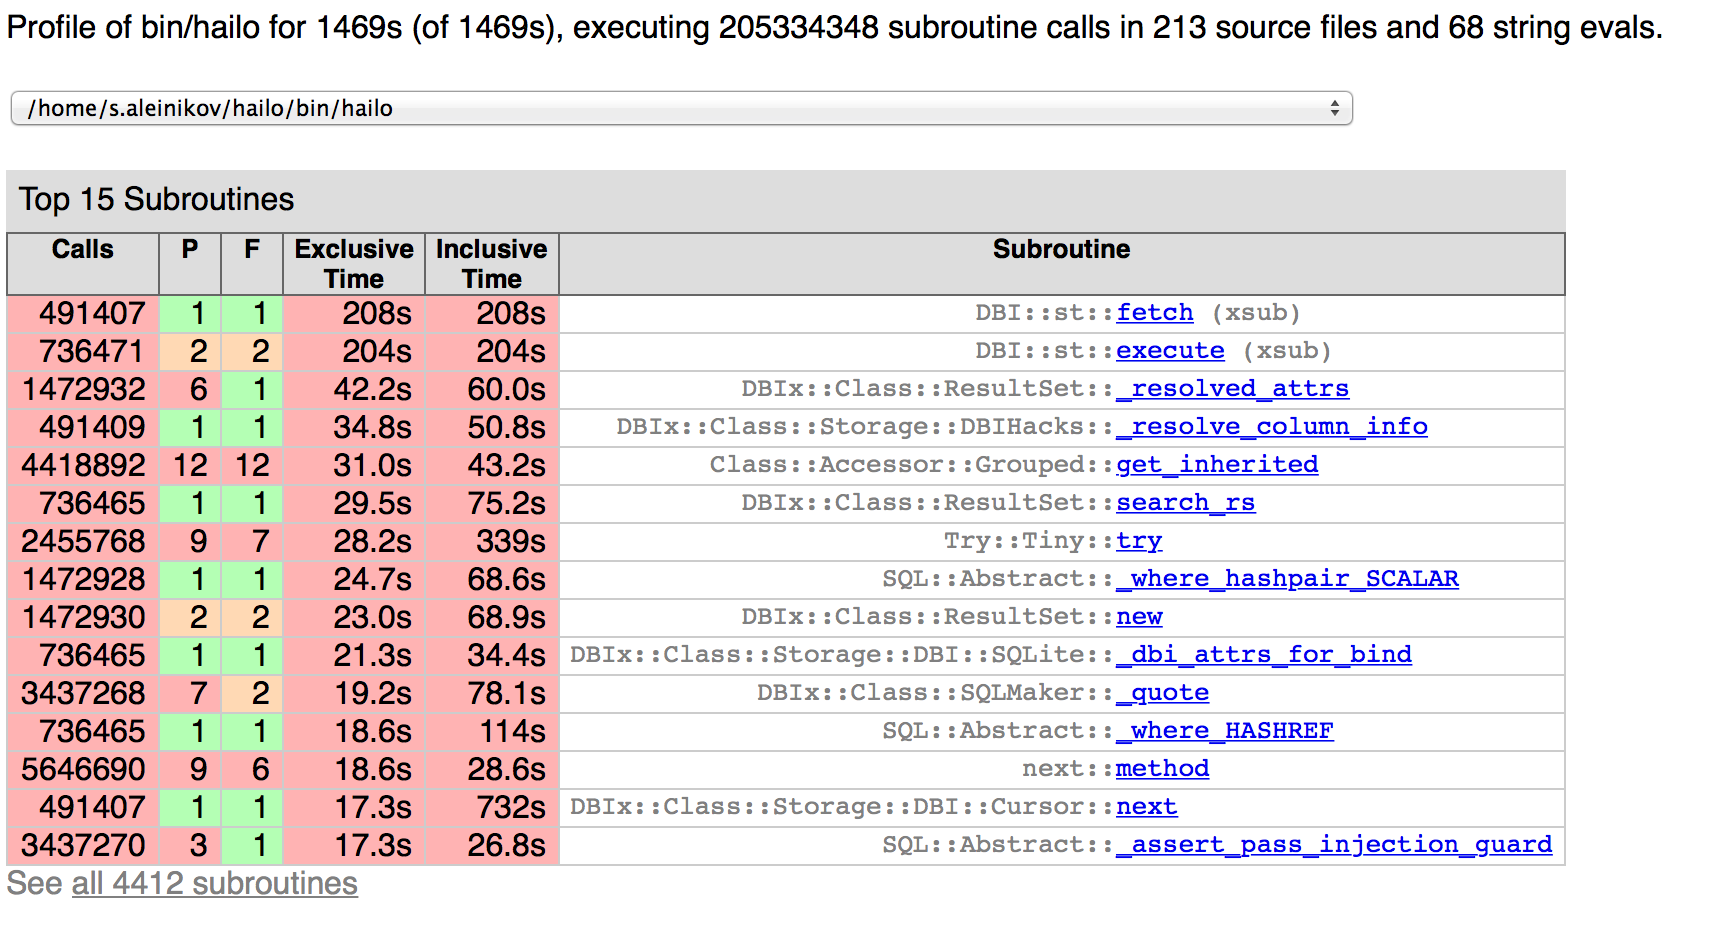
\includegraphics{scr2.png}
}
\end{frame}

\begin{frame}
\scalebox{0.4}{
    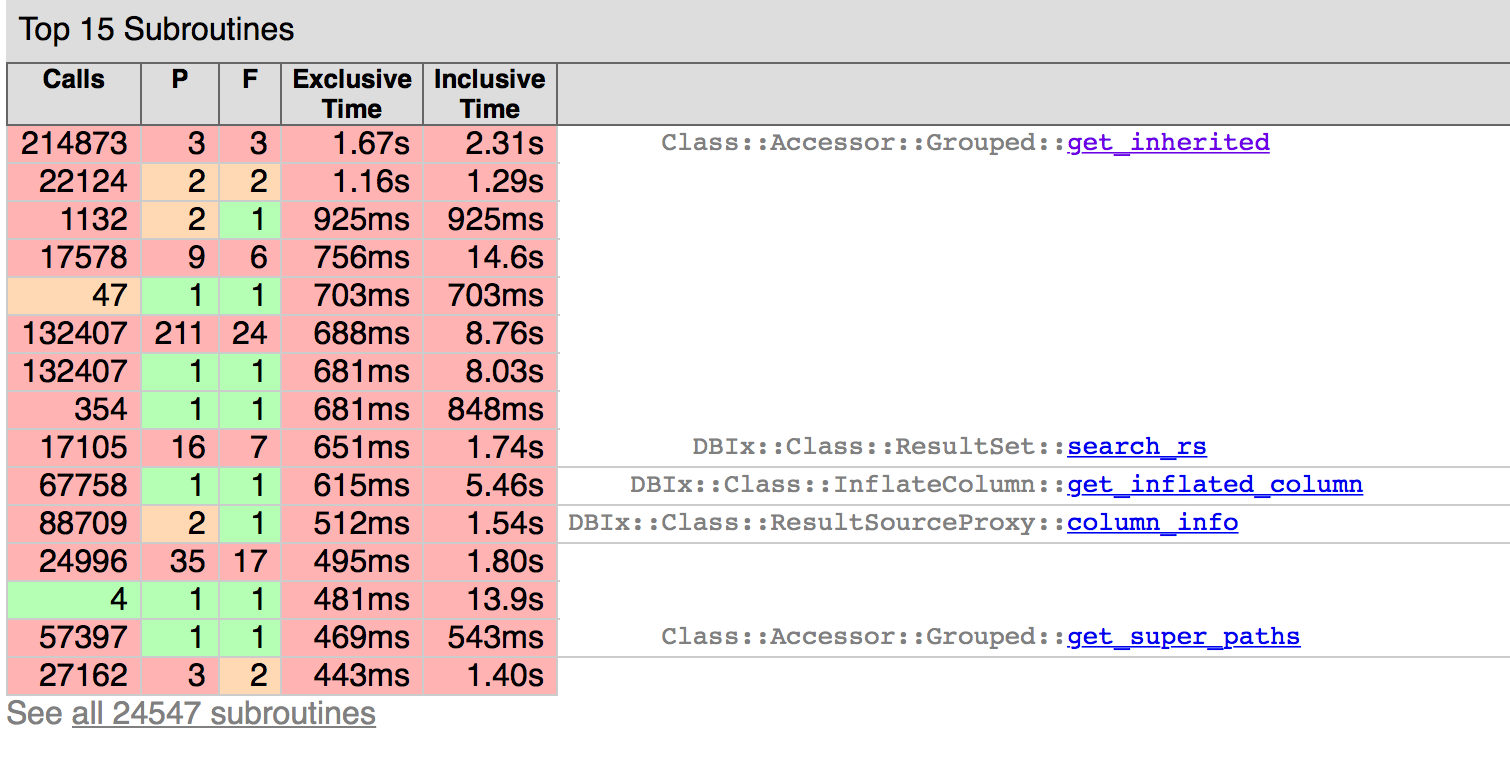
\includegraphics{scr1.png}
}
\end{frame}

{
{
\color{white}
\setbeamercolor{background canvas}{bg=bgc}
\newminted{perl}{fontsize=\fontsize{7}{7}}

\begin{frame}[fragile]
\begin{perlcode}
use CAIXS;

my $LOADED_CACHE = {};
sub _component_class_on_read {
    my $class = $_[0];

    if (defined $class && !blessed($class) && !exists $LOADED_CACHE->{$class}) {
        $LOADED_CACHE->{$class} = undef;
        DBIx::Class::Componentised->ensure_class_loaded($class);
    }

    return $class;
}

sub _inherited_ro_instance_on_write {
    $_[0]->throw_exception("Cannot set value on an instance") if blessed $_[0];
    return $_[1];
}

Class::Accessor::Inherited::XS::register_types(
    component_class       => {read_cb  => \&_component_class_on_read},
    inherited_ro_instance => {write_cb => \&_inherited_ro_instance_on_write},
);
\end{perlcode}
\end{frame}

\begin{frame}[fragile]
\begin{perlcode}
*DBIx::Class::AccessorGroup::mk_group_accessors = sub {
    my ($self, $group, @fields) = @_;
    my $class = ref($self) ? ref($self) : $self;

    state $known_types = {
        inherited               => 'inherited',
        inherited_ro_instance   => 'inherited_ro_instance',
        component_class         => 'component_class',
        simple                  => 'object',
    };

    if (my $type = $known_types->{$group}) {
        Class::Accessor::Inherited::XS::mk_type_accessors($class, $type, @fields);

    } else {
        goto &Class::Accessor::Grouped::mk_group_accessors;
    }
};

*DBIx::Class::mk_classaccessor = sub {
    my ($self, $field) = @_;
    $self->mk_group_accessors('inherited', $field);

    $self->$field($_[2]) if scalar @_ > 2;
};
\end{perlcode}
\end{frame}

}

\begin{frame}
\center{
    Questions?\\
    \vspace{2ex}
    \href{https://github.com/dur-randir/}{https://github.com/dur-randir/}
}
\end{frame}

}\end{document}
